\chapter[Diseño del sistema]{Diseño del sistema}
\label{cap:diseno}

Este capítulo describe \emph{cómo} la plataforma cumple los requerimientos del capítulo anterior.
Siguiendo la recomendación de describir un sistema desde varias vistas \parencite{iso42010}, se presentan la estructura
estática (contenedores), los datos, la red y la seguridad, el comportamiento dinámico (secuencias),
el manejo del tiempo y el despliegue. Las notaciones son las reconocidas en la industria: el modelo
C4 \parencite{c4brown} para la vista de contenedores, diagramas entidad-relación \parencite{chen1976}
para los datos y diagramas de secuencia UML \parencite{uml251} para el comportamiento. Las figuras
se generan automáticamente desde la documentación versionada y, el modelo de datos, desde el esquema
real de la base, de modo que informe, documentación y base no pueden diferir; lo que aún no está
implementado se indica con su etapa.

\section{Vista de contenedores y frontera del trabajo}

La figura~\ref{fig:contenedores} muestra las piezas ejecutables y cómo se comunican; la frontera con
el trabajo del compañero —el tópico MQTT— ya se definió en la sección~\ref{sec:frontera}.

\begin{figure}[!htb]
\centering
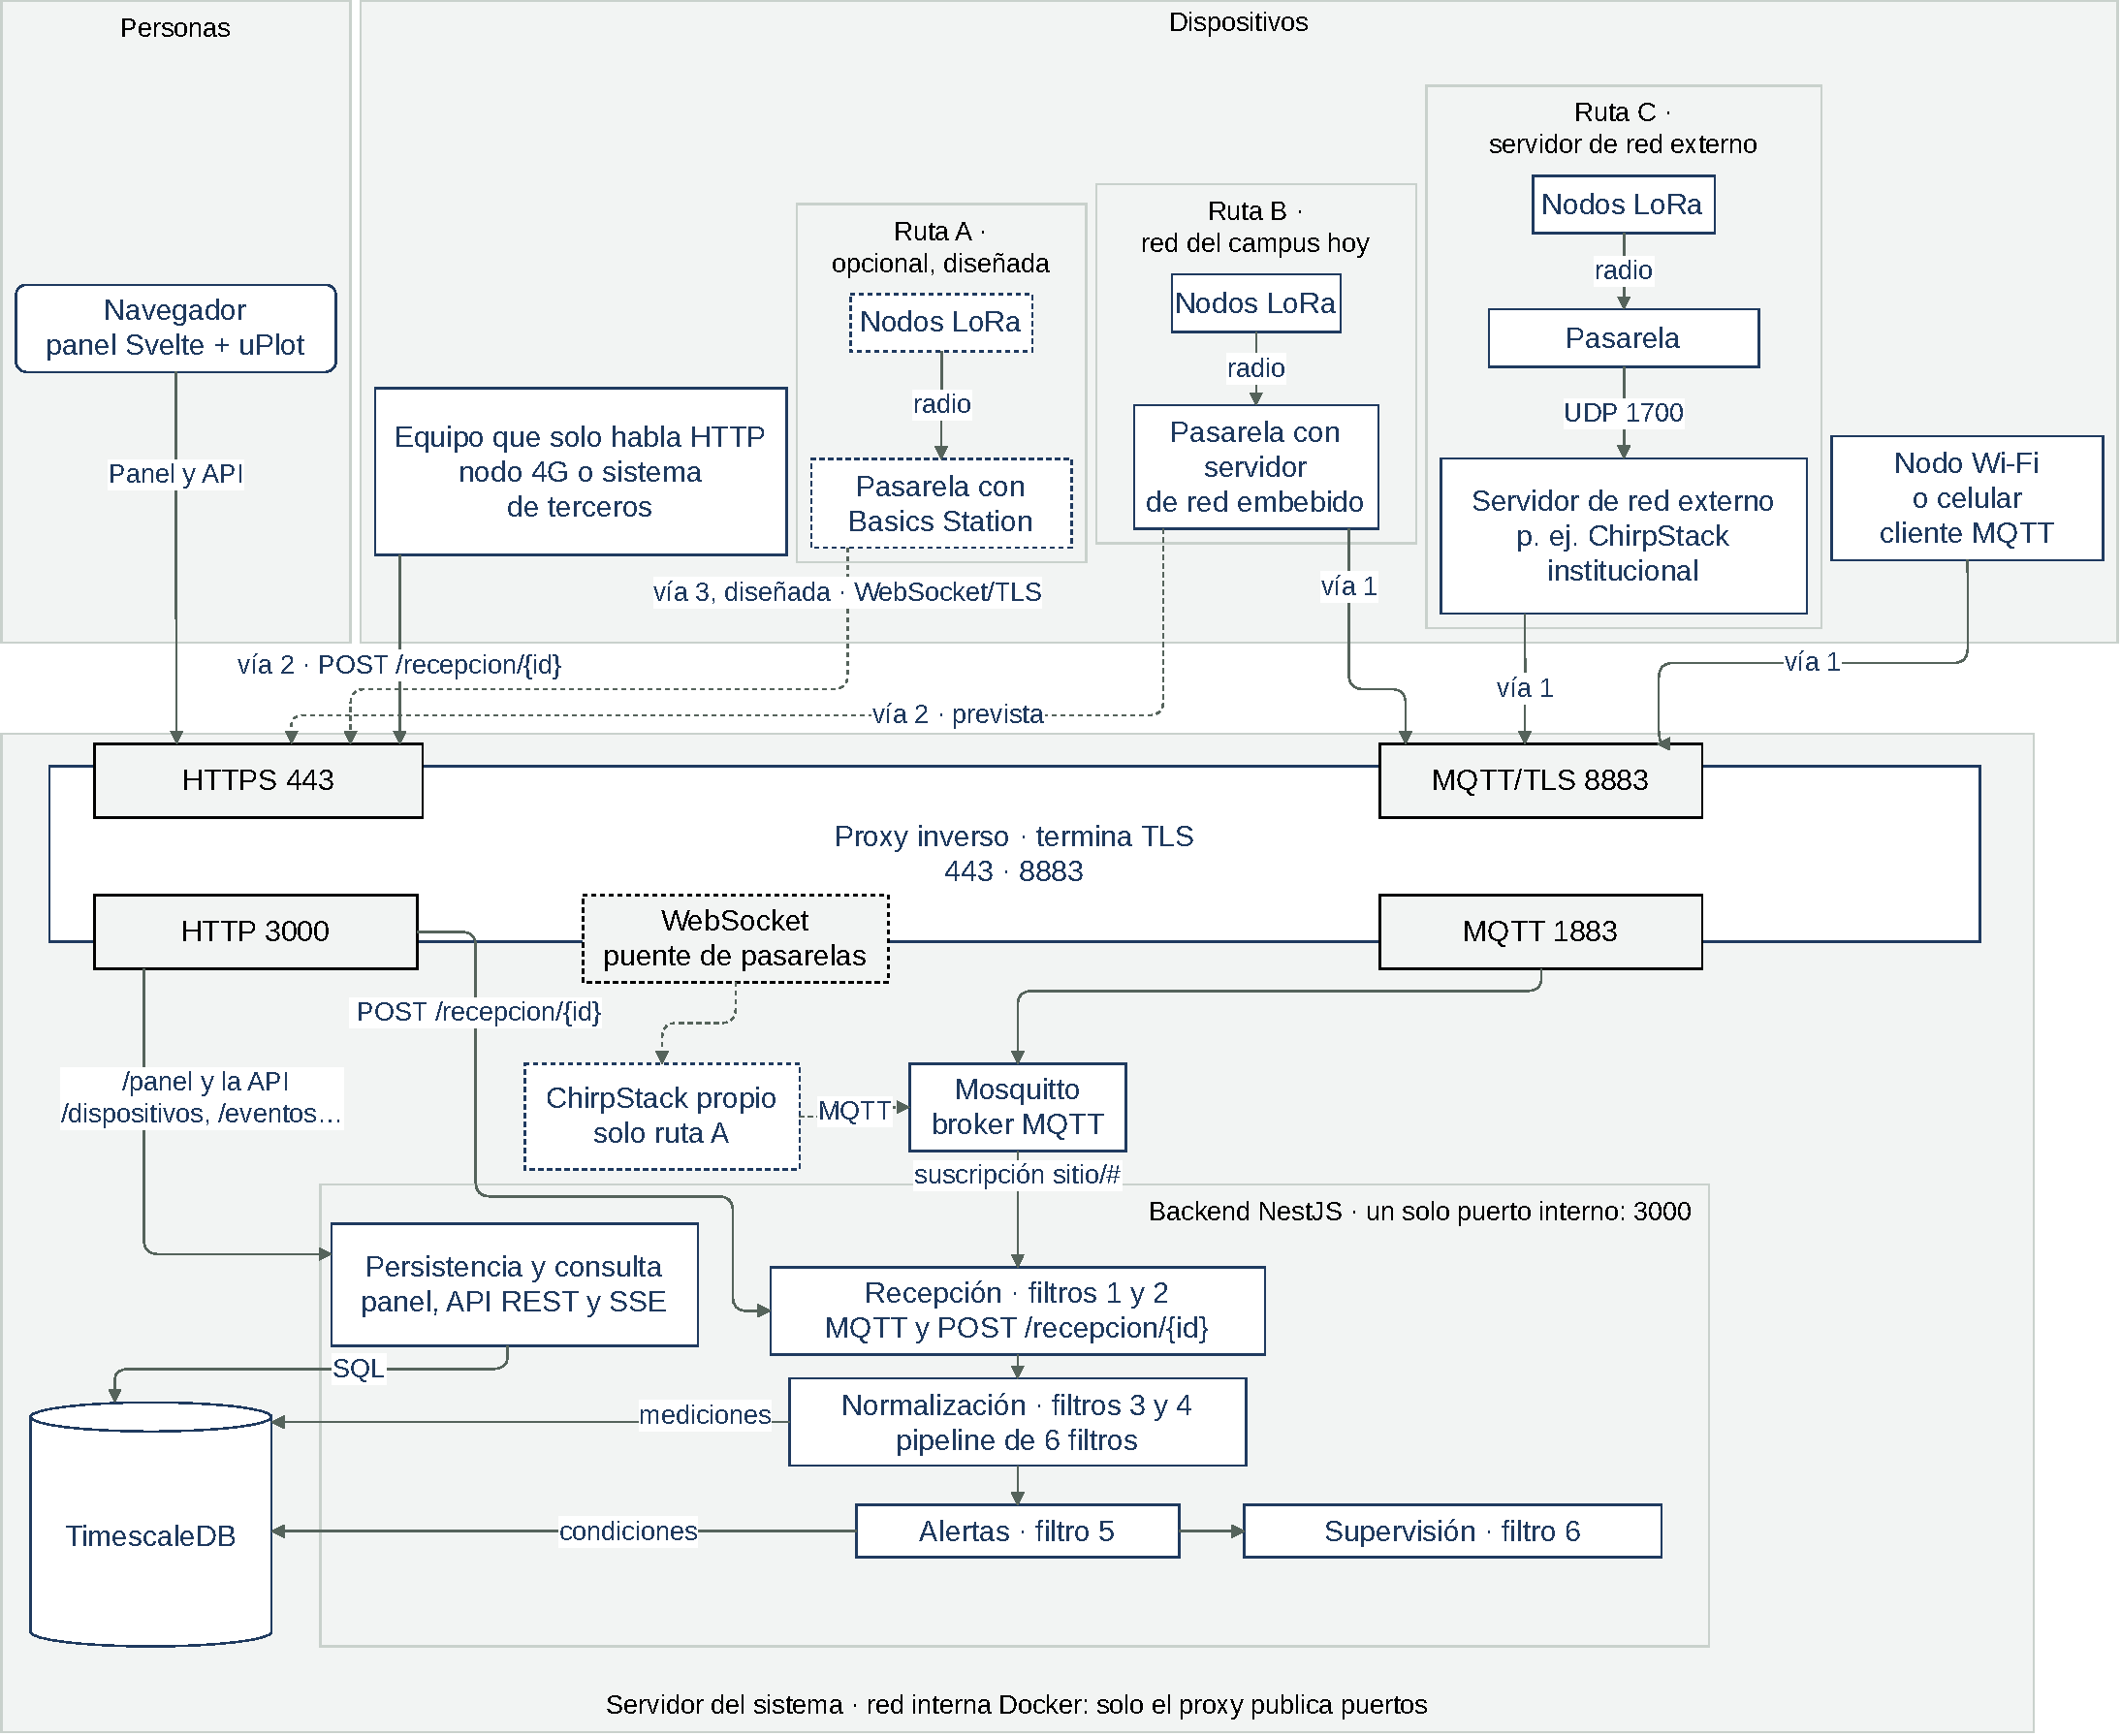
\includegraphics[width=\linewidth,height=0.62\textheight,keepaspectratio]{figuras/drawio/figura-4.1.pdf}
\caption{Vista de contenedores (modelo C4, nivel 2). La frontera del trabajo es el tópico MQTT: de un lado, la red de sensores del compañero (nodos y \emph{gateway}: en la ruta B la pasarela —la red del campus hoy— y en la ruta C un servidor de red externo publican al broker por TLS con su propia credencial (vía 1); en la ruta A, opcional, diseñada y punteada, la pasarela llega por WebSocket sobre TLS con \emph{Basics Station} a un ChirpStack propio (vía 3)); del otro, el proxy —único contenedor expuesto—, el broker y el backend. Un nodo Wi-Fi o celular publica directo por MQTT sobre TLS (vía 1); un equipo que solo habla HTTP entra por 443 con un token (vía 2) y cae en la misma tubería de seis filtros; el reporte HTTPS de la pasarela, variante prevista de la vía 2, va punteado. El navegador nunca se conecta al broker: consume la API del backend, que ya autenticó, validó y normalizó cada trama y, con la sesión de la Etapa 4, cada usuario verá solo los datos de su sitio (RF-41). Las cajas del backend llevan los filtros de la figura~\ref{fig:pipeline} que ejecutan y corresponden a los módulos M1, M2, M6, M4 y M5 del catálogo; M3, M7 y M8 son transversales o viven en el cliente.}
\label{fig:contenedores}
\end{figure}


Tres decisiones quedan visibles en la figura. Primero, hay \textbf{dos puntos de entrada siempre y tres a lo
sumo}: HTTPS para personas (443), MQTT sobre TLS para dispositivos y pasarelas de las rutas B y C (8883) y, solo
en la ruta A, opcional y punteada, UDP para los \emph{gateways} LoRaWAN (1700). Ese tercer puerto recibe un
protocolo sin autenticación ni cifrado propios (\emph{Semtech UDP Packet Forwarder}), así que la defensa
la dan el contenedor sin privilegios y el límite de tasa, no el protocolo. La base de datos y la
consola de administración de ChirpStack nunca se exponen. Segundo, \textbf{el navegador nunca se conecta al
broker}: consume la API del backend, que ya autenticó, validó y normalizó cada trama. La alternativa
—suscribir el navegador al broker por WebSocket— habría expuesto el broker a Internet y puesto
credenciales MQTT en el código del cliente. Tercero, \textbf{el servidor de red LoRaWAN es un productor más} hacia el
broker: una trama LoRaWAN decodificada y una trama Wi-Fi directa son indistinguibles para la
plataforma después del filtro de análisis, que es lo que resuelve la causa C2 (hardware atado a la
plataforma).

Los ocho módulos del análisis (capítulo~\ref{cap:especificacion}) se reparten así: M1 recepción y M2
normalización forman el servicio de recepción del backend, es decir, el pipeline; M4 supervisión de
salud es el barrido periódico; M5 persistencia y consulta es la API sobre TimescaleDB; M6 alertas es el
servicio de umbrales. No aparecen como cajas M3 inventario y aprovisionamiento ni M7 seguridad e
identidad, transversales al backend y previstos para la siguiente etapa, ni M8 interfaz, que es el
panel y corre en el navegador.

\section{Modelo de datos}

El modelo (figura~\ref{fig:modelo-datos}) tiene 18 entidades y una idea rectora: \textbf{el modelo
interno es único}. No importa por qué vía ni en qué formato llegó una trama; una vez superado el
pipeline, todo se guarda con la misma forma. Esa uniformidad es la respuesta a la causa C1 (formatos
dispares). El esquema está en tercera forma normal, y no más allá porque la cuarta y la quinta resuelven dependencias multivaluadas y de reunión que este modelo no tiene: cada hecho vive en una sola tabla y las
relaciones muchos a muchos se resuelven con entidades de asociación (\texttt{canal} es dispositivo por
magnitud; \texttt{usuario\_sitio}, usuario por sitio). Las únicas redundancias son deliberadas y se
llaman «foto por valor»: la unidad copiada en cada medición y el umbral vigente copiado en cada evento,
para que cambiar un catálogo no reinterprete el pasado.

\begin{figure}[!tbp]
\centering
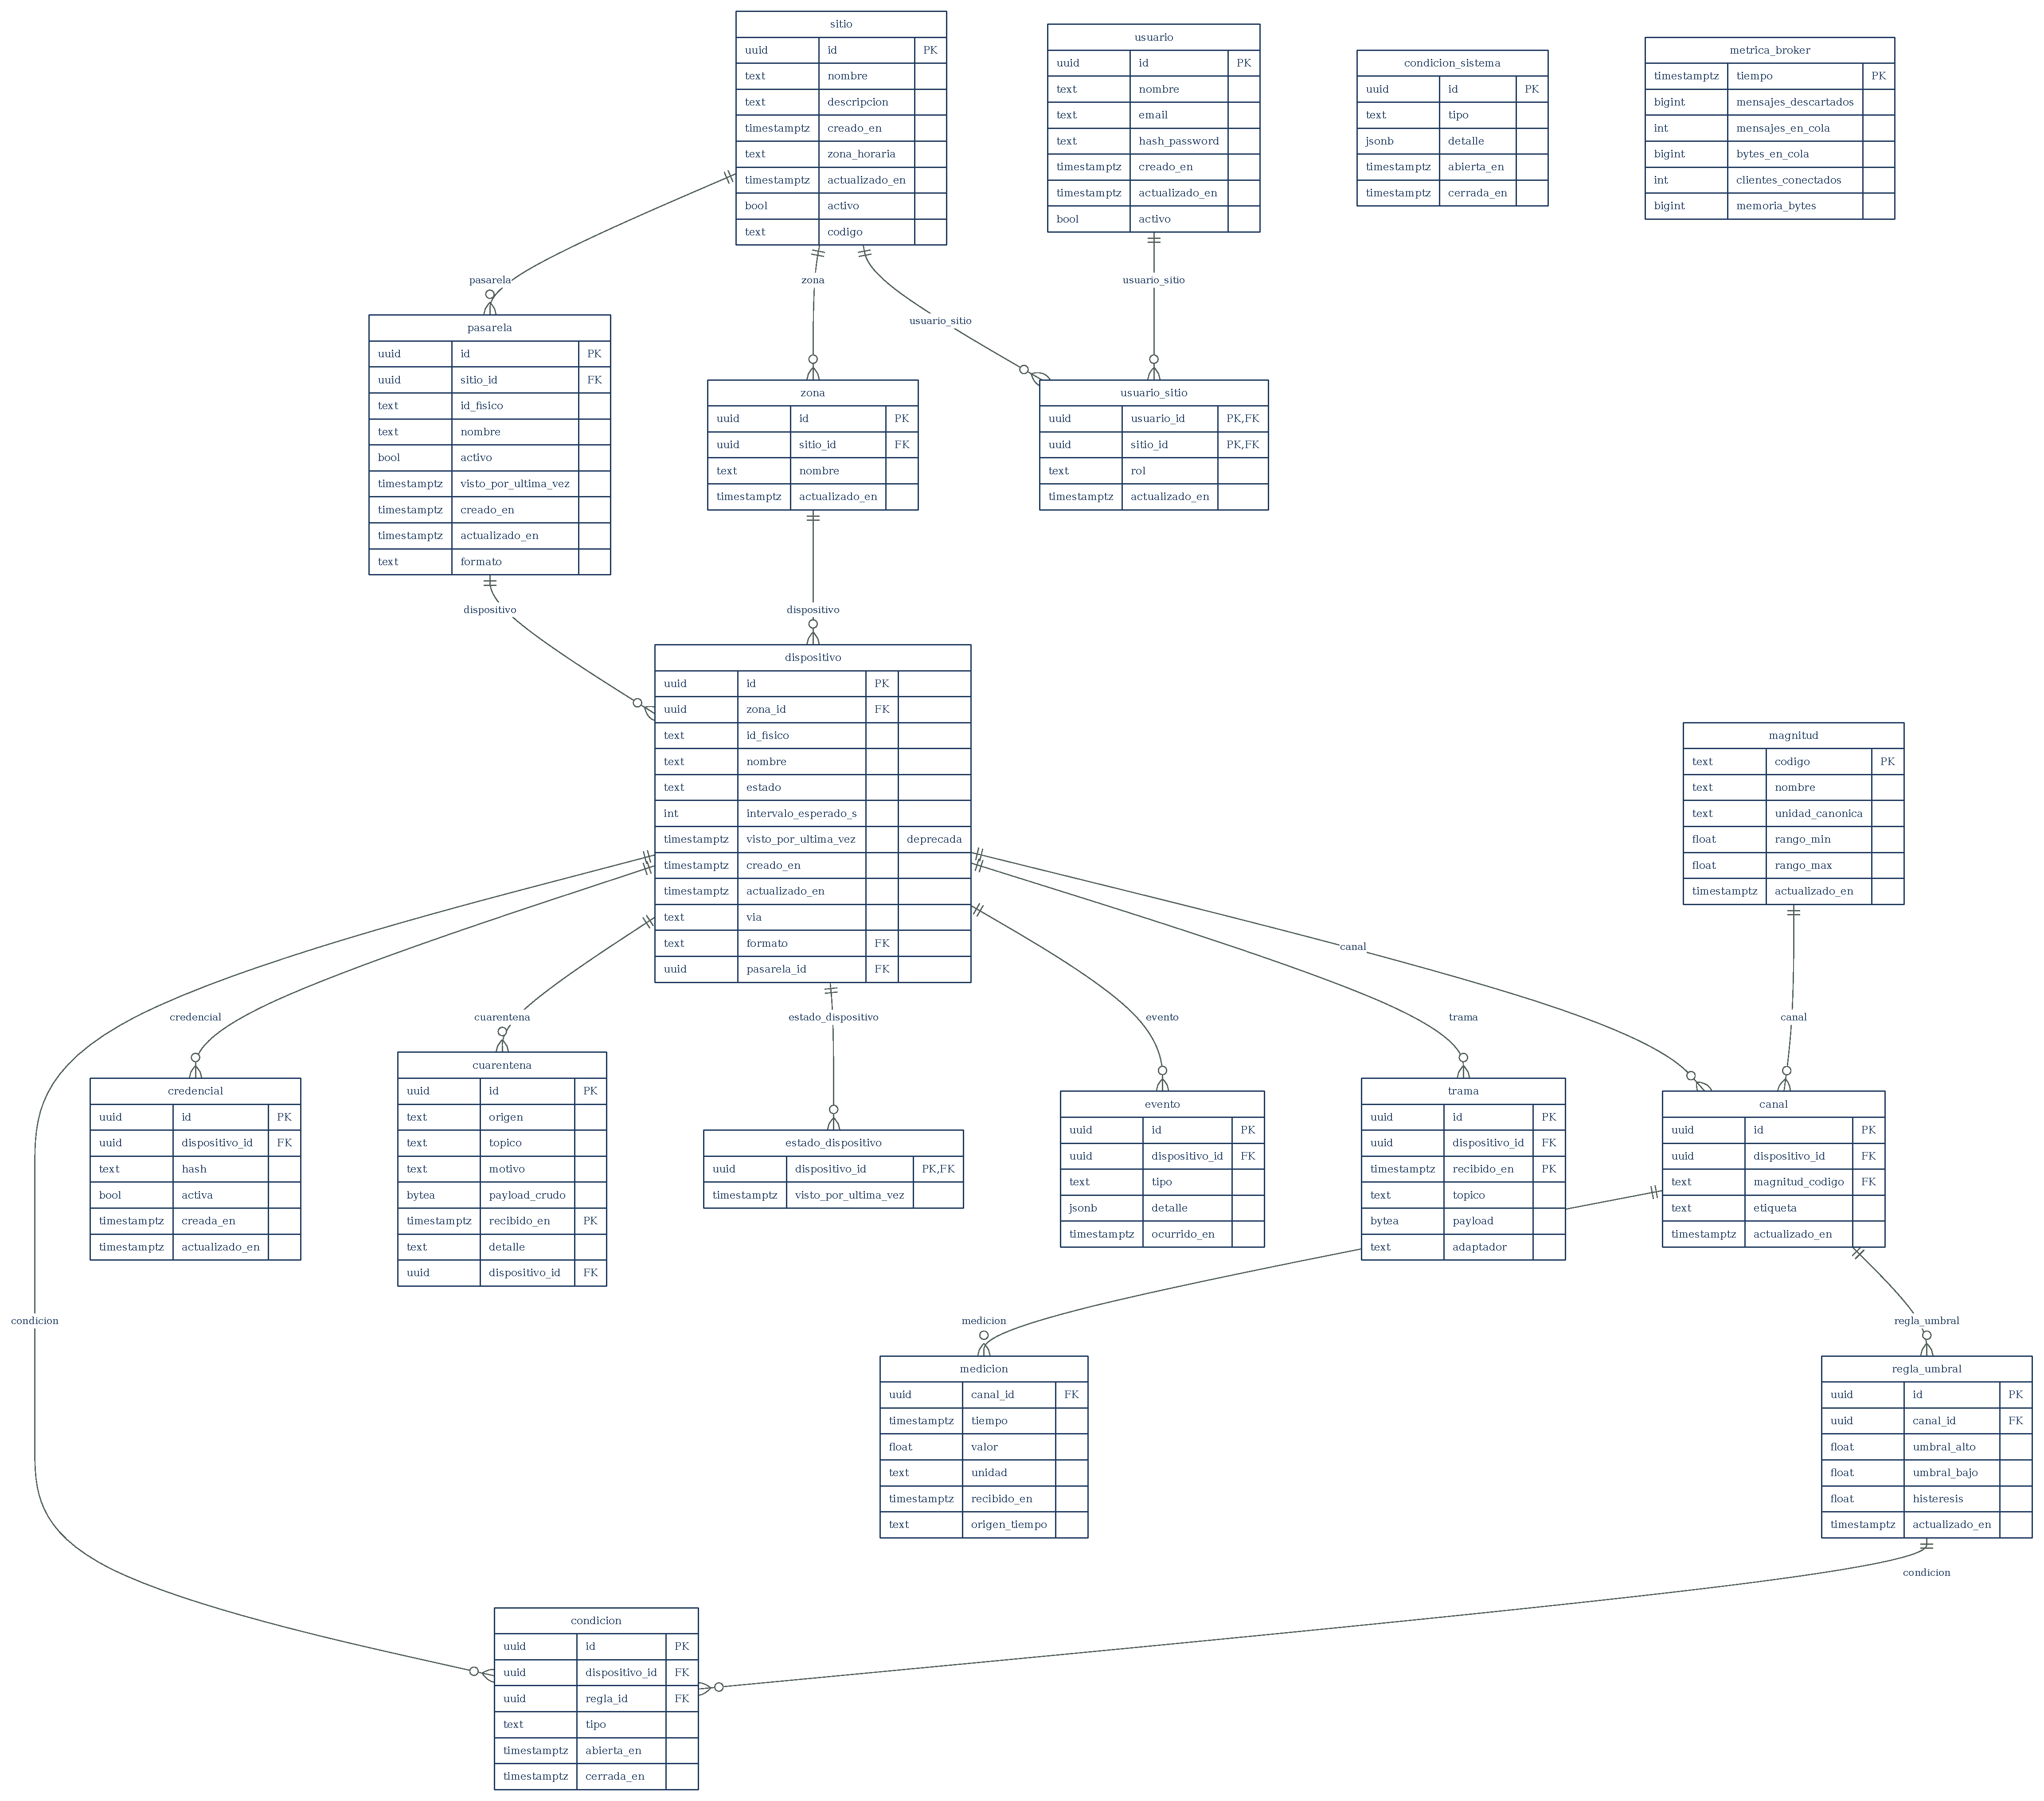
\includegraphics[width=\linewidth,height=0.74\textheight,keepaspectratio]{figuras/render/modelo-datos.pdf}
\caption[Modelo de datos, generado desde el esquema real]{Modelo de datos (diagrama entidad-relación, notación \emph{crow's foot}), generado desde el esquema real de la base de datos. 22 entidades: la organización (\texttt{sitio}, \texttt{zona}, \texttt{usuario} y \texttt{usuario\_sitio}), el acceso de las personas (\texttt{sesion} y \texttt{acceso}), lo propio de cada una (\texttt{preferencia} y \texttt{mensaje\_soporte}), el inventario (\texttt{dispositivo}, \texttt{pasarela}, \texttt{canal}, \texttt{credencial}, \texttt{estado\_dispositivo} y el catálogo \texttt{magnitud}), las series de tiempo (\texttt{medicion}), el estado (\texttt{regla\_umbral}, \texttt{condicion}, \texttt{evento}), lo crudo ---\texttt{trama}, aceptada, y \texttt{cuarentena}, rechazada y atribuida al dispositivo cuando se sabe cuál es--- y la salud del propio sistema (\texttt{condicion\_sistema}, \texttt{metrica\_broker}). \texttt{medicion}, \texttt{trama}, \texttt{cuarentena}, \texttt{metrica\_broker} y \texttt{acceso} son hypertables particionadas por tiempo. Una medición pertenece a un \emph{canal} —dispositivo más magnitud— y no al dispositivo: un nodo que mide temperatura y humedad produce dos series.}
\label{fig:modelo-datos}
\end{figure}



Las decisiones del modelo y su justificación —por qué la medición cuelga del canal, por qué la credencial es una entidad aparte, por qué la cuarentena vive aparte de las series— se detallan en el cuadro~\ref{tab:decisiones-datos} (anexo~\ref{anx:evaluacion}). Lo que el diagrama no muestra por convención también está diseñado: el esquema sigue un conjunto de \textbf{convenciones de calidad} verificadas contra la base real —toda restricción con nombre explícito y prefijo (\texttt{pk\_}, \texttt{fk\_}, \texttt{uq\_}, \texttt{ck\_}), un índice por cada clave foránea (PostgreSQL no lo crea solo y sin él cada unión recorre la tabla completa), auditoría con \texttt{actualizado\_en} mantenida por disparador en toda tabla mutable, baja lógica en lugar de borrado, dominios cerrados como \texttt{CHECK} y catálogos donde el usuario administra los valores, y comentarios \texttt{COMMENT ON} en las columnas cuya razón de ser no es obvia, de modo que la documentación viaja con la base—. El esquema evoluciona por \textbf{migraciones numeradas} (\texttt{01-esquema}, \texttt{02} unicidad
de condición por regla, \texttt{03} zona horaria por sitio, \texttt{04} serialización uniforme de
instantes, \texttt{05} convenciones de calidad, \texttt{06} clave natural única de la serie, \texttt{07} dominio cerrado de \texttt{cuarentena.motivo}): nunca se edita un archivo ya aplicado. Una instalación nueva ejecuta todas en orden; una
base existente aplica solo las nuevas.

\section{Topología de red y seguridad en capas}

La figura~\ref{fig:red} (anexo~\ref{anx:figuras}) muestra los tres segmentos de red y qué cruza cada frontera. Los dispositivos
del sitio abren únicamente \textbf{conexiones salientes}, de modo que el router del cliente no necesita
puertos abiertos ni configuración alguna (RNF-10): una organización sin personal técnico (causa C4)
conecta un sensor sin tocar su red.


La seguridad se diseñó en capas, asumiendo en cada una que la anterior falló: (1)~red: solo 443, 8883
y 1700/udp publicados; (2)~TLS obligatorio en producción; (3)~identidad: broker sin conexiones anónimas,
usuario MQTT igual al identificador físico, contraseñas con hash; (4)~lista de control de acceso (ACL) por
patrón: cada dispositivo escribe solo bajo su propio identificador, lo que impide la suplantación entre
nodos; (5)~el pipeline valida y envía a cuarentena; (6)~datos: base sin puerto expuesto, una credencial
por servicio; (7)~contenedores sin escalada de privilegios, con versión de imagen fijada y techo de
recursos; (8)~operación: respaldos, secretos fuera del repositorio. Las capas 1, 3, 4, 5 y 7 están
implementadas y \textbf{verificadas} en el despliegue de desarrollo: una publicación anónima o con clave
incorrecta es rechazada, y un dispositivo que intenta publicar en el tópico de otro es descartado sin
que el suscriptor llegue a recibir el mensaje.

\section{Comportamiento}

\subsection{Aprovisionamiento de un dispositivo}

La figura~\ref{fig:sec-alta} (anexo~\ref{anx:figuras}) describe cómo un dispositivo pasa de desconocido a reconocido. Es el flujo que ataca la causa C4: una persona sin perfil técnico registra un dispositivo, hoy por la API y desde el panel en la Etapa~4; según la vía declarada, el sistema genera la credencial, la muestra \textbf{una vez}, guarda su hash y registra
al dispositivo en el broker con una lista de acceso restringida a su propio tópico. El estado «en línea»
no nace del alta, sino del \textbf{primer mensaje autenticado}.


\subsection{Recepción de una trama: el pipeline}

La figura~\ref{fig:sec-pipeline} (anexo~\ref{anx:figuras}, apaisada para que se lea) detalla el aporte central del trabajo, organizado según el patrón
\emph{pipes and filters} \parencite{posa1}. Cada filtro tiene una salida que
continúa y una de rechazo hacia la cuarentena; ninguna lectura llega a las series sin superar los cuatro
primeros, y los dos últimos no escriben series sino condiciones.
El orden importa: autenticar primero evita gastar recursos en tramas de desconocidos; validar antes de
guardar evita que una lectura imposible llegue a la serie. Los dos últimos filtros trabajan a distinta escala: el de alertas
evalúa \emph{cada lectura} guardada, porque un umbral se cruza por valor; el de supervisión se ejecuta
\emph{una vez al cerrar la trama}, porque lo que registra no es un dato sino un hecho del enlace —este
dispositivo se comunicó—, y por eso marca al dispositivo como visto aunque sus lecturas hayan ido a
cuarentena: un nodo que publica tramas malformadas está vivo y mal configurado, no en silencio, y
confundir ambos casos manda al operador a buscar la falla donde no está. El filtro de análisis delega en \textbf{adaptadores} intercambiables —SenML
\parencite{rfc8428} como contrato nativo y un formato plano para nodos simples—, de modo que admitir el formato de un nuevo
fabricante es agregar una clase, no modificar el pipeline (RF-04). La entrega desde el broker es
«al menos una vez»: QoS~1 con sesión persistente, de modo que si el backend cae el broker conserva la
cola, hasta un tope de mensajes, y la entrega al volver. Eso admite reentregas, y por ello la inserción en la serie es idempotente
sobre la clave natural canal e instante: una lectura repetida se ignora sin volver a evaluar umbrales
(RF-06, RF-10). No se usa QoS~2: su garantía vale por salto cliente–broker \parencite{mqttoasis}, no
hasta la base; el receptor debe ser idempotente igual y, con eso, QoS~1 basta.


Un detalle de diseño que no se ve en la secuencia: el pipeline solo corre \emph{cuando llega} una trama,
así que no puede notar que un dispositivo \emph{dejó} de transmitir. Por eso existe un \textbf{supervisor
periódico} (M4) que compara la última recepción de cada dispositivo con su intervalo esperado y abre la
condición «sin comunicación» cuando el silencio supera dos intervalos. Un mensaje perdido no es una
caída; dos seguidos, sí. Las alertas por umbral (M6) usan \textbf{histéresis}: la condición abre al cruzar
el umbral y cierra solo al volver un margen más adentro, para que un valor que oscila alrededor del
límite no dispare y cierre alertas sin parar.

\subsection{Panel en tiempo real}

La figura~\ref{fig:sec-tiemporeal} (anexo~\ref{anx:figuras}) muestra los dos tiempos del panel. El histórico llega
\textbf{agregado por la base de datos} con \texttt{time\_bucket}: cientos de puntos, no millones. Las lecturas
nuevas las empuja el backend por un canal SSE, cifrado tras el proxy, que solo anuncia
lo ya guardado, rechaza otro origen u otro host y limita los flujos abiertos; desde la Etapa~4 se abre con la sesión del
panel, como recomienda OWASP para WebSocket \parencite{owaspws}. El navegador nunca toca el broker. Toda consulta valida sus entradas (identificadores, fechas, un intervalo de una lista
cerrada) y usa parámetros, nunca texto interpolado. El \textbf{contrato de la API se
genera desde el código}, en OpenAPI 3.0 \parencite{openapi303}, desde los controladores, así no puede describir rutas
inexistentes; se sirve junto a la API y se versiona como el acuerdo que consumirá el panel.


\section{Despliegue y presupuesto de recursos}

La figura~\ref{fig:despliegue} (anexo~\ref{anx:figuras}) muestra el despliegue: un servidor, una red interna y
cuatro contenedores —proxy, broker, backend y base de datos—, más ChirpStack solo en la ruta A, con una
base propia dentro del mismo PostgreSQL. El backend no guarda estado, por lo que puede recrearse sin pérdida. Cada contenedor tiene versión de imagen
fijada, no puede escalar privilegios, se reinicia solo ante fallas y tiene un techo de memoria y CPU.


La suma de techos es de 1,6~GB en la ruta B —los cuatro contenedores ya implementados— y de
1,95~GB con ChirpStack (ruta A), ambas dentro del RNF-17 (consumo de a lo más 2~GB de RAM); el consumo real se
mide en la Etapa~4. Los
límites cumplen además una segunda función: definen el \textbf{entorno de referencia} del banco de pruebas
de la Etapa~4, para que la comparación no dependa del equipo de desarrollo.

\textbf{Alojamiento.} La recomendación es un \textbf{servidor privado virtual (VPS) internacional de 2~vCPU y 4~GB},
del orden de CLP~6\,000 mensuales, para la validación y un primer sitio, con un VPS nacional como alternativa si se
exigen datos en Chile. La comparación de cinco alternativas con precios fechados y el costo por retención están en el
anexo~\ref{anx:evaluacion} (cuadro~\ref{tab:alojamiento}).

\textbf{Tiempo.} Todo instante se guarda en UTC y cada sitio declara su zona por nombre (\texttt{America/Santiago}):
como Chile cambia de hora por decreto, toda pregunta de «día» se responde dentro de la base, en la zona del sitio
(reglas y verificación en el anexo~\ref{anx:evaluacion}, sección~\ref{sec:tiempo}).

\textbf{Trazabilidad.} Cada elemento de diseño materializa requerimientos del catálogo
(cuadro~\ref{tab:trazabilidad-diseno}, anexo~\ref{anx:evaluacion}); RF-29 queda pendiente: el backend aún no
publica \emph{Last Will}.
